
\documentclass[10pt,conference]{IEEEtran}

\usepackage[T1]{fontenc}
\usepackage[utf8]{inputenc}

\usepackage{amsmath}
\usepackage{amssymb}
\usepackage{booktabs}
\usepackage{array}
\usepackage{tabularx}
\usepackage{graphicx}
\usepackage[table]{xcolor}
\usepackage{url}
\usepackage{cite}
\usepackage{balance}
\usepackage{multirow}

\usepackage[hidelinks]{hyperref}

\newcommand{\dataset}{\textsc{LangWarrant}}
\newcommand{\metric}[1]{\textsc{#1}}


\begin{document}

\title{[Experiment, Analysis, and Benchmark] \dataset: Evaluating Response-Language Authorization in Multilingual Workflow Prompts}

\author{\IEEEauthorblockN{Anonymous Author(s)}
\IEEEauthorblockA{Anonymous Institution}}

\maketitle


\begin{abstract}
Multilingual workflow prompts often expose several plausible language cues, including source records, user turns, internal notes, recipient profiles, policies, and output schemas. In such settings, response language is not merely generated from the most salient context; it should be authorized by the workflow evidence item that controls the current output. We introduce \dataset{}, a 1,500-instance benchmark organized into 500 controlled warrant triads for evaluating \emph{language-warrant selection}. Each triad separates sensitivity to true warrant changes from robustness against non-authoritative shortcut cues. Across six primary LLM evaluation runs, task completion remains high, at or above 0.900, while triad-level warrant consistency ranges from 0.108 to 0.968. These results show that models can complete workflow tasks while binding the response language to the wrong visible cue, exposing a recurring failure mode in multilingual workflow evaluation.
\end{abstract}

\begin{IEEEkeywords}
multilingual instruction following, language warrant, workflow evaluation, benchmark construction, LLM evaluation
\end{IEEEkeywords}


\section{Introduction}

Multilingual workflow prompts rarely ask a model to choose an output language in isolation. They combine source records, internal notes, recipient profiles, policies, and output schemas into a single model-visible context. These contexts often expose several plausible language cues at once: the latest user turn may be written in one language, the source record in another, and the recipient-facing contract in a third. In such settings, response language is an authorization decision over workflow evidence, rather than a preference among visible languages. \emph{Visible language cues are not language warrants.} The model must identify which evidence item has authority for the current output. A model can recognize every visible language span, produce a task-complete response, and still produce an unauthorized output if it follows a salient but non-authoritative cue. Our main evaluation shows that this failure is not marginal: across six primary LLM evaluation runs, task completion is always at least 0.900, while a stricter triad-level measure of warrant consistency ranges from 0.108 to 0.968.

Consider a customer-support record containing source content in Korean, internal context in English, and a selected recipient-facing locale field in Spanish. All three fields are visible to the model, and all three expose language information. Only one of them authorizes the response language for the current task. The Korean source content and English internal context are visible language cues, but neither licenses the customer-facing response; the selected Spanish recipient-facing field does. A model that follows the Korean source content or the English internal context may produce a plausible and task-relevant output, but the output is unauthorized because it follows a shortcut cue rather than the operative warrant. Figure~\ref{fig:warrant-selection} summarizes this cue-warrant conflict.

\begin{figure*}[t]
\centering
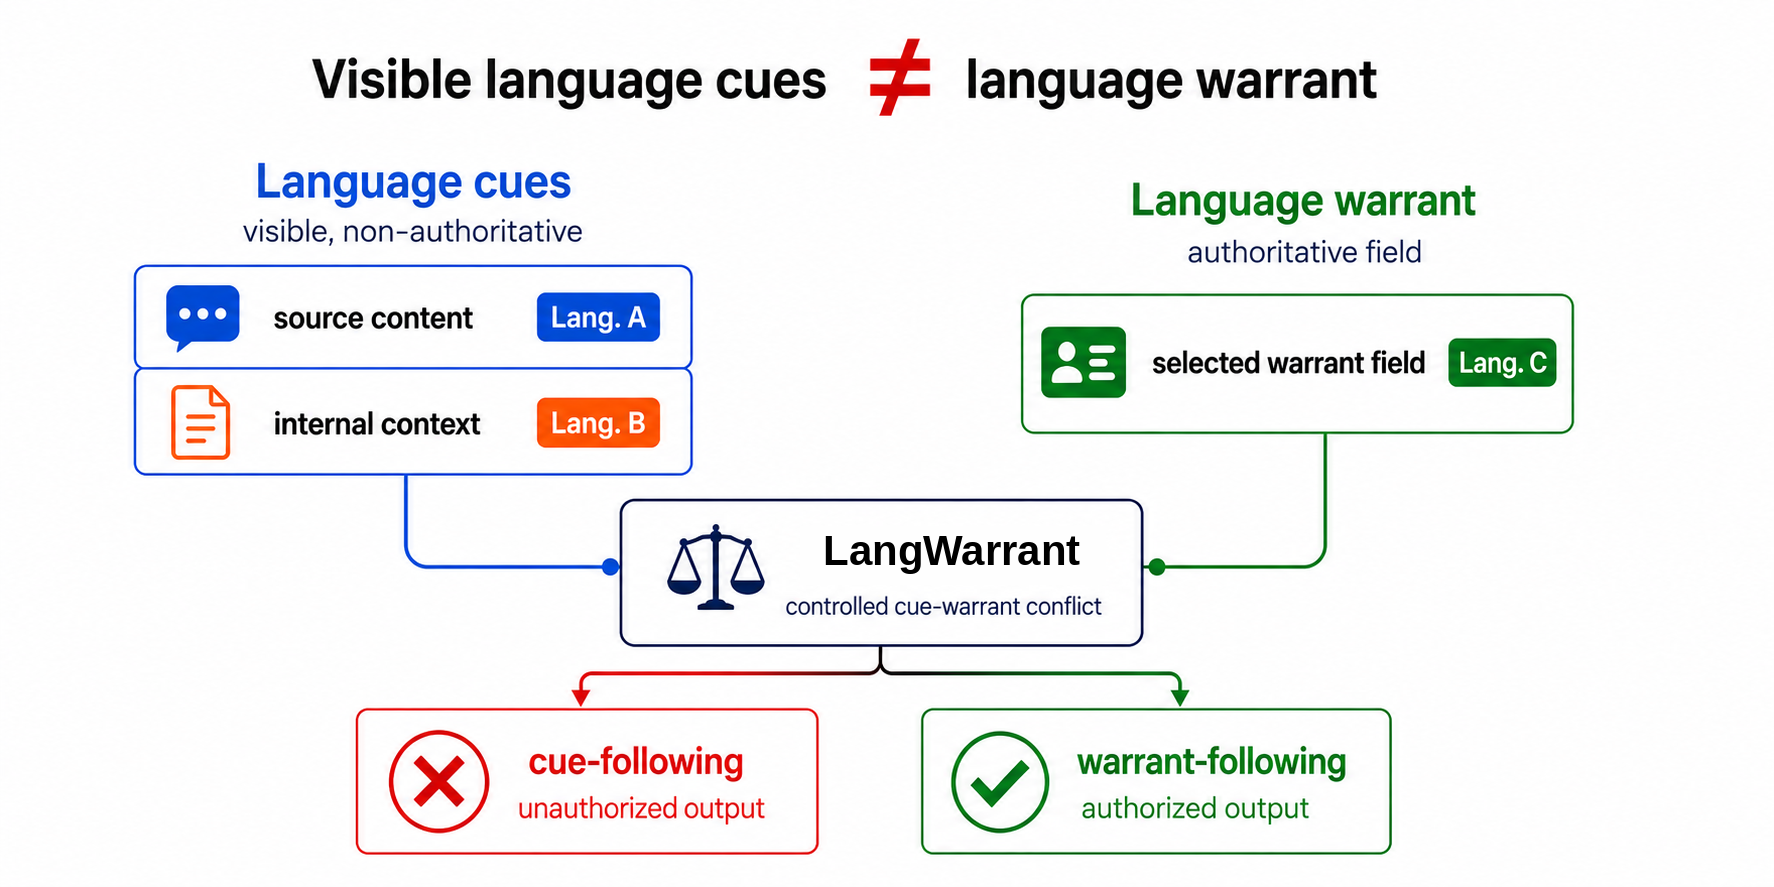
\includegraphics[width=\textwidth]{figures/fig1_language_warrant_selection.png}
\caption{Language-warrant selection under competing workflow cues. A multilingual workflow prompt may contain multiple language-bearing fields, but only the selected warrant field authorizes the response language for the current task. \dataset{} evaluates whether models follow the warrant rather than shortcut cues.}
\label{fig:warrant-selection}
\end{figure*}

We call the authoritative evidence that licenses the response language a \emph{language warrant}. A language warrant is not hidden from the model; it is a model-visible workflow evidence item whose authority is specified by the task contract, selected field, policy, recipient profile, or output schema. The distinction is authority, not visibility. Throughout the paper, \emph{authorization} is defined with respect to this benchmark workflow contract; it is not a claim about legal, institutional, or organizational authority outside the prompt. A language cue is any visible language-bearing signal in the prompt, whereas a language warrant is the evidence item that should control the response language for the current workflow. \emph{Language-warrant selection} is the decision problem of selecting that operative warrant under competing visible cues and then generating in the language licensed by it. A wrong-language response in this setting is therefore an evidence-selection failure, not only a surface language-generation failure.

The warrant framing also has a narrow sociolinguistic motivation. Language choice in communicative settings depends on participant roles, audience, domains, and policy regimes, rather than on the mere presence of a language in context \cite{fishman1965who,hymes1974foundations,bell1984audience,spolsky2004languagepolicy}. \dataset{} operationalizes this idea as a benchmark object: the response language should follow the workflow evidence item that has standing for the current output surface.

Existing multilingual evaluations leave a coverage mismatch rather than a generic absence of multilingual tests. One line of work treats language as an axis of task transfer: cross-lingual benchmarks ask whether task competence carries across languages, so the target language is part of the benchmark condition rather than an evidence item to be selected at inference time \cite{hu2020xtreme}. A second line studies response-language stability under multilingual prompting. These studies show that models can drift toward recent, salient, or contextually dominant language cues, but the controlling language is still defined as an intended or requested language, not as the output of an authority-selection problem among workflow fields \cite{marchisio2024languageconfusion,zhang2024respond}. Recent multilingual RAG evaluations add an explicit evidence channel and show that retrieved content in another language can pull generation away from the desired response language \cite{li2026ragdrift}. However, retrieval language in these settings is primarily a contextual influence, not a controlled non-authoritative distractor paired with a separately selected warrant. Multilingual instruction-following benchmarks further test whether models satisfy language-conditioned task constraints across languages and mixed-language inputs \cite{dussolle2025mifeval}. They still do not isolate the workflow case where multiple visible fields contain plausible language cues, only one field is authorized to determine the response language, and the non-authoritative fields are deliberately varied as shortcut controls. The missing evaluation unit is therefore not another target-language label, but a controlled workflow cell: one field authorizes the response language, other visible language-bearing fields act as shortcuts, one perturbation should change the authorized language, and another should not. Without these controls, an item-level wrong-language output remains under-specified: it may indicate weak cross-lingual competence, ordinary language drift, instruction-following failure, or selection of the wrong authoritative evidence. \dataset{} fills this coverage mismatch by making warrant fields, shortcut cues, warrant shifts, distractor shifts, and triad-level response patterns first-class evaluation objects.

A single prompt instance cannot reliably reveal whether a model follows a warrant or merely matches a salient language cue. \dataset{} therefore uses controlled warrant triads: a base item, a warrant-shift item, and a distractor-shift item. The warrant shift changes the operative warrant and should change the target language; the distractor shift changes salient non-controlling cues while preserving the authorized language. This design separates warrant sensitivity from shortcut robustness. The release contains 1,500 instances organized into 500 triads, supporting both item-level scoring and triad-level analysis of cue-warrant conflicts.

Auditability in \dataset{} follows from the task definition. In language-warrant selection, the label is an authority claim: it specifies which model-visible evidence item may determine the response language. Data-validation work treats such assumptions as explicit benchmark invariants \cite{breck2019datavalidation}, and data-centric benchmark work emphasizes exposing the conditions under which measurements are meaningful \cite{mazumder2023dataperf}. \dataset{} therefore stores each warrant decision with its provenance, including the selected warrant field and licensing evidence span. Following dataset-documentation and provenance principles, these records support audits of whether a wrong-language output reflects model-side warrant selection, annotation error, or scorer interpretation \cite{gebru2021datasheets,herschel2017provenance}.

Applying \dataset{} reveals a strong separation between task completion and warrant-consistent triad behavior. Across six primary evaluation runs, all models complete the requested task at high rates, with task-completion scores at or above 0.900, yet triad-level warrant consistency ranges from 0.108 to 0.968. The weakest runs therefore do not primarily fail by producing empty, malformed, or task-irrelevant outputs. They often preserve the requested structure and complete the business task while repeatedly binding the response language to a salient shortcut cue rather than to the operative warrant. We do not interpret the arithmetic difference between item-level and triad-level scores as a standalone failure mass, because the triad score is deliberately conjunctive. Instead, the empirical point is that high task completion and plausible individual outputs can coexist with low group-level reliability under warrant and distractor controls.

We make the following contributions:
\begin{itemize}
\item \textbf{Problem formulation.} We define language-warrant selection as a workflow evidence-selection problem in multilingual LLM evaluation, where wrong-language outputs may reflect non-authoritative evidence selection rather than language generation failure alone.
\item \textbf{Benchmark design.} We introduce \dataset{}, a 1,500-instance benchmark organized into 500 controlled warrant triads that separate warrant sensitivity from shortcut robustness.
\item \textbf{Auditable annotations.} We release warrant provenance, selected evidence spans, shortcut roles, triad roles, and fixed scorer contracts, making warrant labels and scorer decisions inspectable.
\item \textbf{Empirical finding.} Across six primary LLM evaluation runs, task completion remains at or above 0.900, while triad-level warrant consistency ranges from 0.108 to 0.968, showing that task completion and controlled warrant-consistent behavior can separate sharply.
\end{itemize}


\section{Benchmark Positioning and Related Evaluation Lines}

\dataset{} is positioned against adjacent evaluation lines by asking what each line treats as the unit of evaluation. Prior work already covers cross-lingual task transfer, wrong-language generation, multilingual instruction following, mixed-language processing, structured tool or schema compliance, and benchmark governance. The remaining coverage mismatch is narrower: existing benchmarks rarely make the authority-bearing workflow field the object being selected and scored.


\begin{table*}[t!]
\caption{Coverage matrix for response-language authorization.}
\label{tab:benchmark-positioning}
\centering
\footnotesize
\setlength{\tabcolsep}{4.2pt}
\renewcommand{\arraystretch}{1.10}
\begin{tabularx}{\textwidth}{@{}p{0.24\textwidth}>{\raggedright\arraybackslash}X>{\centering\arraybackslash}p{0.11\textwidth}>{\centering\arraybackslash}p{0.12\textwidth}>{\centering\arraybackslash}p{0.11\textwidth}>{\centering\arraybackslash}p{0.11\textwidth}@{}}
\toprule
\multirow{2}{*}{\raisebox{0.55ex}{\textbf{Evaluation line}}} &
\multirow{2}{*}{\raisebox{0.55ex}{\textbf{Main target}}} &
\multicolumn{4}{c}{\textbf{Coverage of response-language warrant selection}} \\
\cmidrule(lr){3-6}
&
&
\textbf{Auth. field} &
\textbf{Non-auth. cue} &
\textbf{Warrant shift} &
\textbf{Matched group} \\
\midrule
Cross-lingual benchmarks &
Task transfer &
No &
No &
No &
No \\
Wrong-language failure &
Intended-language match &
Implicit &
Partial &
No &
No \\
RAG drift &
Source-language pull &
Implicit &
Partial &
Partial &
No \\
Instruction following &
Constraint satisfaction &
Instruction &
Limited &
No &
No \\
Code-switching &
Mixed-language processing &
N/A &
Partial &
No &
No \\
Tool/schema compliance &
Schema or API compliance &
Partial &
Partial &
No &
No \\
Benchmark governance &
Release documentation &
N/A &
N/A &
N/A &
N/A \\
\midrule
\textbf{\dataset{}} &
\textbf{Response-language authorization} &
\textbf{Yes} &
\textbf{Yes} &
\textbf{Yes} &
\textbf{Yes} \\
\bottomrule
\end{tabularx}

\vspace{0.25em}
\begin{minipage}{0.98\textwidth}
\scriptsize
\textit{Note.}
Auth. field denotes an explicit response-language field with standing under the task contract.
Non-auth. cue denotes controlled language-bearing cues that should not determine the final response language.
Warrant shift denotes counterfactual variation in the authority-bearing field.
Matched group denotes group-level scoring over paired or triadic controls.
Rows summarize representative evaluation lines cited in the surrounding text rather than exhaustively classifying all work in each area.
\end{minipage}
\end{table*}


\textbf{Cross-lingual competence is not workflow authorization.}
XTREME frames multilingual evaluation as cross-lingual generalization over a multi-task benchmark, so its primary unit is task transfer across languages rather than the selection of an authority-bearing workflow field \cite{hu2020xtreme}. Belebele makes reading comprehension parallel across 122 language variants, which strengthens cross-lingual comparability while still fixing the evaluated language condition through the benchmark design \cite{bandarkar2024belebele}. These benchmarks are central references for multilingual capability evaluation, but their target language is normally specified by the task, dataset, or evaluation condition. \dataset{} evaluates a different decision point: whether the model can infer the response language from the workflow evidence item that is authorized to license it.

\textbf{Language confusion work identifies the failure mode but usually presupposes the target language.}
Marchisio et al. study language confusion as a multilingual LLM failure in which the model answers in an unintended language, establishing wrong-language generation as a measurable reliability problem \cite{marchisio2024languageconfusion}. Zhang et al. focus on response-language inconsistency and the problem of making models respond in the user-intended language \cite{zhang2024respond}. Li et al. move this failure mode into multilingual retrieval-augmented generation, where retrieved source documents can pull generation away from the desired response language \cite{li2026ragdrift}. These studies motivate \dataset{}, but they mostly evaluate whether generation matches an intended language after that intention has been specified, implied, or induced by the input setting. \dataset{} shifts the unit of evaluation one step earlier: the model must first identify which visible workflow field has authority to define the intended language.

\textbf{Multilingual instruction-following benchmarks test constraint satisfaction, not warrant selection.}
M-IFEval adapts instruction-following evaluation to multilingual settings, making verifiable constraint satisfaction across languages the main object of measurement \cite{dussolle2025mifeval}. MaXIFE extends this line toward multilingual and cross-lingual instruction-following evaluation, emphasizing whether models can satisfy instructions across language conditions \cite{liu2025maxife}. Marco-Bench-MIF further targets multilingual instruction-following behavior as a benchmarked capability rather than treating language choice as a workflow authorization problem \cite{zeng2025marco}. M2Lingual focuses on multilingual, multi-turn instruction alignment, which is especially relevant to dialogue-like settings but still evaluates alignment to instructions rather than selection among competing authority-bearing fields \cite{maheshwary2025m2lingual}. This line is mature and directly adjacent to \dataset{}. The distinction is that \dataset{} does not ask only whether a language-conditioned instruction is followed. It asks whether the model can determine which visible field has the standing to impose that language condition.

\textbf{Code-switching and mixed-language benchmarks evaluate mixed linguistic material as the target phenomenon.}
GLUECoS evaluates code-switched NLP across tasks, treating code-switching itself as the linguistic condition under which systems must operate \cite{khanuja2020gluecos}. LinCE provides a centralized benchmark for linguistic code-switching evaluation, again making mixed-language text the evaluated object \cite{aguilar2020lince}. CodeMixBench extends code-mixing evaluation to LLMs across 18 languages, testing whether models can handle or produce mixed-language behavior \cite{yang2025codemixbench}. \dataset{} uses multilingual prompts differently. Mixed languages are not the target linguistic phenomenon to be processed. They are competing evidence sources inside a workflow, only one of which authorizes the final response language.

\textbf{Structured-output and data-centric work supply the release discipline.}
ToolLLM and StableToolBench foreground evaluation under explicit tool, API, schema, and execution contracts, providing a contract-oriented analogue for field-level evaluation \cite{qin2024toolllm,guo2024stabletoolbench}. DataPerf and data-validation work treat data definitions, validation, and task contracts as first-order evaluation objects, showing that benchmark quality depends on more than aggregate model scores \cite{mazumder2023dataperf,breck2019datavalidation}. Dataset documentation, provenance, and versioning work further motivate explicit records of dataset purpose, composition, transformations, intended use, reuse conditions, and artifact evolution \cite{gebru2021datasheets,pushkarna2022datacards,herschel2017provenance,bhattacherjee2015datasetversioning}. \dataset{} uses this literature as release discipline rather than as its task construct: the task construct is response-language authorization, while the release records preserve selected warrant fields, evidence spans, distractor cues, triad roles, scorer contracts, validation outputs, repair records, manifests, checksums, and audit addenda so that each response-language authority claim remains inspectable.


\section{\dataset{} Design}

\dataset{} is built to evaluate response-language authorization in workflow prompts where multiple language cues are visible at the same time. The benchmark does not treat the target response language as a free-standing class label. Instead, the target language is derived from a selected warrant field, namely the model-visible evidence item that has authority over the response language for the current task. Other language-bearing fields remain present in the prompt and may be locally plausible, but they are non-authoritative shortcuts.

This section defines the benchmark object in five steps. We first describe the instance-level data object and task contract. We then summarize the construction and validation pipeline used to produce the frozen release. We next introduce the controlled warrant triad, which is the main construction unit. We then describe warrant sources, difficulty strata, and release statistics. Finally, we state the benchmark scope and the intended interpretation of results.

\subsection{Data object and task contract}

Each \dataset{} instance contains a workflow input, a language warrant, and an evaluation contract. The workflow input is the model-visible task context: it may include source content, operator notes, customer or recipient metadata, routing state, channel information, policy fields, and output-format requirements. The selected warrant field identifies the evidence item that authorizes the response language. Warrant evidence spans record the exact field value or text span supporting that decision. Distractor cues record visible language-bearing signals that a shortcut-following model might incorrectly select. The evaluation contract specifies which output surface is scored and which task-completion or format guards apply.

This representation separates three objects that are often collapsed in multilingual evaluation: a visible language cue, an authoritative warrant, and the derived target language. For example, a workflow record may contain Korean source material, an English operator note, and a Spanish recipient locale. The target response language is Spanish only when the recipient locale is the selected warrant field. The Korean and English spans still matter because they create shortcut pressure, but they do not authorize the final response language.

The benchmark includes task and format requirements because warrant selection is evaluated in workflow settings rather than isolated translation prompts. Some instances ask for customer-facing replies or portal messages; others require structured payloads, CRM notes, notification bundles, or visible/internal field separation. These constraints allow later scoring to separate wrong-language behavior from empty, malformed, or task-irrelevant outputs.


\subsection{Construction and validation pipeline}

The frozen release was constructed as a controlled benchmark object rather than collected as natural traffic. Table~\ref{tab:construction-pipeline} summarizes the construction path. Seed workflow patterns define domains, task types, output formats, and candidate language-bearing fields. Each pattern is instantiated into a base workflow record with one selected warrant field and one or more non-authoritative language cues. The base record is then expanded into a triad by applying two counterfactual edits: a warrant edit that changes the authorized language and a distractor edit that changes a salient non-authoritative cue while preserving the authorized language.

\begin{table}[t]
\caption{Construction and validation pipeline for the frozen release.}
\label{tab:construction-pipeline}
\centering
\scriptsize
\setlength{\tabcolsep}{3.2pt}
\renewcommand{\arraystretch}{1.08}
\begin{tabularx}{\columnwidth}{@{}>{\raggedright\arraybackslash}p{0.25\columnwidth}>{\raggedright\arraybackslash}p{0.35\columnwidth}>{\raggedright\arraybackslash}X@{}}
\toprule
\textbf{Stage} & \textbf{Object produced} & \textbf{Validation gate} \tabularnewline
\midrule
Pattern seeding & workflow family, task format, candidate warrant fields & domain facts and task contract are explicit \tabularnewline
Base instantiation & model-visible workflow record & selected warrant field and evidence span are present \tabularnewline
Triad expansion & base, warrant-shift, distractor-shift items & warrant edit changes gold language; distractor edit preserves it \tabularnewline
Contract attachment & LF, TC, format, and field-policy rules & scorer-visible metadata is separated from model input \tabularnewline
Integrity filtering & frozen 500 valid triads & schema validity, span grounding, role balance, and shortcut controls pass \tabularnewline
Audit and freeze & v1.0 release plus v0.2k scorer & repair replay, regression replay, and human audit bounds are recorded \tabularnewline
\bottomrule
\end{tabularx}
\end{table}

All model-visible prompts are paired with evaluator-only metadata. The model receives only the workflow input. The hidden metadata records the target response language, selected warrant field, warrant evidence spans, distractor cues, task-completion rule, format rule, and field-language policy. This separation is necessary because revealing the selected warrant or gold language would turn the benchmark into direct instruction following. Integrity gates remove items whose selected warrant is not span-grounded, whose triad edit breaks the required language relation, or whose distractor change creates a second plausible warrant rather than a non-authoritative cue.

\subsection{Controlled warrant triads}

The core construction unit is a controlled warrant triad. Each triad contains a base item, a warrant-shift item, and a distractor-shift item. The base item establishes an initial relation among the selected warrant, the visible shortcut cues, and the gold response language. The warrant-shift item changes the operative warrant and therefore changes the gold response language. The distractor-shift item changes a salient non-authoritative cue while preserving the operative warrant and the gold response language. Figure~\ref{fig:controlled-triad} illustrates the triad as a compact behavioral test.

\begin{figure}[t]
\centering
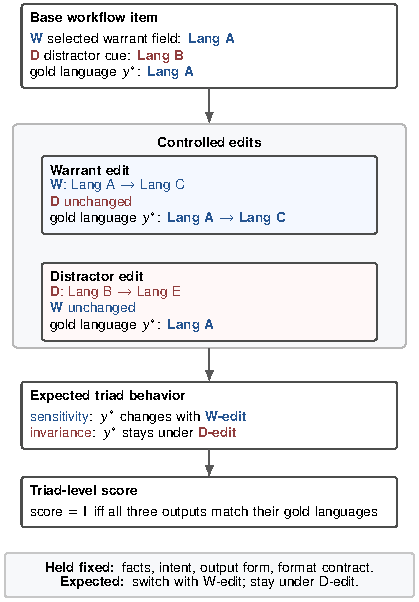
\includegraphics[width=0.94\columnwidth]{figures/fig2_triad_design.pdf}
\caption{Controlled warrant triad design. A base workflow item is paired with a warrant edit and a distractor edit. W-edit denotes the warrant-shift edit, and D-edit denotes the distractor-shift edit. The expected behavior is sensitivity to warrant changes and invariance to distractor-only changes; a triad receives credit only when all three outputs match their gold languages.}
\label{fig:controlled-triad}
\end{figure}

The triad structure turns response-language choice into an evidence-selection problem. Item-level target-language accuracy can show whether a single output uses the expected language, but it cannot determine whether the model followed the warrant or merely matched a salient cue. The warrant-shift item tests sensitivity to the controlling evidence. The distractor-shift item tests invariance under shortcut pressure. A model must satisfy both conditions within the same triad: it should change language when the warrant changes and remain stable when only a non-authoritative cue changes.

A triad is therefore scored more strictly than three independent items. It receives credit only when all three outputs match their gold languages. This criterion does not claim access to the model's internal causal reasoning. It evaluates whether the observable response pattern is consistent with warrant following under controlled perturbations.

\begin{table}[t]
\caption{Example controlled triad from the frozen release.}
\label{tab:example-triad}
\centering
\scriptsize
\setlength{\tabcolsep}{3.0pt}
\renewcommand{\arraystretch}{1.08}
\begin{tabularx}{\columnwidth}{@{}>{\raggedright\arraybackslash}p{0.24\columnwidth}>{\raggedright\arraybackslash}p{0.32\columnwidth}>{\raggedright\arraybackslash}p{0.29\columnwidth}>{\centering\arraybackslash}X@{}}
\toprule
\textbf{Triad role} & \textbf{Warrant-bearing field} & \textbf{Visible non-warrant cue} & \textbf{Gold} \tabularnewline
\midrule
Base & \texttt{priorThread.locale = en-US} & source language = ja; \texttt{contextLocale = es-ES} & en \tabularnewline
Warrant shift & \texttt{priorThread.locale = fr-FR} & same source and context locale & fr \tabularnewline
Distractor shift & \texttt{priorThread.locale = en-US} & \texttt{contextLocale = ko-KR} & en \tabularnewline
\bottomrule
\end{tabularx}
\vspace{0.25em}
\begin{minipage}{0.98\columnwidth}
\scriptsize
This example is a compact view of frozen group G026. The business fact is held fixed: notification time is 09:00 and SMS remains disabled. The warrant-shift edit changes the active thread locale; the distractor-shift edit changes only a non-selected context locale.
\end{minipage}
\end{table}

Table~\ref{tab:example-triad} shows the local logic of a real frozen triad. The base and distractor-shift rows both license English because the active recipient-thread locale remains \texttt{en-US}. The warrant-shift row licenses French because the same active field changes to \texttt{fr-FR}. The context locale is visible and language-bearing, but it is not authorized to determine the response language for this workflow action.


\subsection{Warrant sources and difficulty strata}

\dataset{} covers warrant sources that occur in workflow-style prompts, including explicit user instructions, customer or recipient language preferences, policy-selected contact locales, active outbound surfaces, schema-visible locale policies, channel states, document fields, and structured-output contracts. These sources are deliberately heterogeneous: some warrants are stated directly, while others must be recovered from workflow state, policy selection, or output-surface constraints.

Difficulty strata increase the distance between a visible language cue and the operative authority. L0 items use direct language instructions. L1 items use local recipient or customer preferences. L2 items require following a policy-selected or profile-selected locale rather than a salient source language. L3 items make the active channel, outbound surface, or workflow route determine the authorized language. L4 items add structured-output pressure, such as nested fields, visible/internal separation, CRM notes, portal messages, secure-inbox payloads, arrays, and schema-visible locale policies.

The strata are construction levels, not a psychometric scale with equal distance between adjacent levels. Their role is to organize increasingly indirect warrant evidence and stronger shortcut pressure. This design supports controlled analysis by warrant source, workflow complexity, and output format.


\begin{table}[t]
\caption{Dataset snapshot for the frozen \dataset{} release.}
\label{tab:dataset-statistics}
\centering
\scriptsize
\setlength{\tabcolsep}{4.0pt}
\renewcommand{\arraystretch}{1.38}
\newcommand{\tabstat}[2]{%
\begin{tabular}[c]{@{}c@{}}
\textbf{#1}\\[0.18em]
#2
\end{tabular}%
}
\begin{tabular}{@{}lccc@{}}
\toprule
& \textbf{Scale} & \textbf{Warrant control} & \textbf{Coverage} \\
\midrule
\textit{Core} &
\tabstat{1,500}{instances} &
\tabstat{500}{valid triads} &
\tabstat{8}{target languages} \\
\midrule
\textit{Quality} &
\tabstat{1,500}{unique item IDs} &
\tabstat{0}{invalid triads} &
\tabstat{180 to 193}{items per language} \\
\midrule
\textit{Design} &
\tabstat{500 / 500 / 500}{base / warrant / distractor} &
\tabstat{8}{warrant families} &
\tabstat{5}{difficulty strata} \\
\midrule
\textit{Workflow} &
\tabstat{360}{L4 items} &
\tabstat{visible/internal}{field separation} &
\tabstat{nested outputs}{CRM / portal / arrays} \\
\bottomrule
\end{tabular}
\end{table}


Table~\ref{tab:dataset-statistics} gives a compact snapshot of the frozen release. The central design property is warrant control: the dataset contains 500 valid triads with balanced base, warrant-shift, and distractor-shift roles. The release also combines near-balanced target-language coverage, multiple warrant-source families, five difficulty strata, and structured workflow settings. These properties support the benchmark's main goal: separating response-language authorization from ordinary task completion, format following, or source-language copying.

All experiments in this paper use the frozen 1,500-instance release. During release alignment, the model-visible task content, target response languages, selected warrant fields, warrant evidence spans, distractor cues, workflow families, difficulty strata, structured-output policies, and format rules were preserved. Intermediate construction batches are not treated as evaluation objects. The paper-facing benchmark name is \dataset{}. Frozen item identifiers and some artifact filenames retain the legacy internal prefix \texttt{SLD\_v1\_0} to preserve checksums and provenance links from the release process. The artifact manifest records this alias explicitly rather than rewriting frozen identifiers after scoring.

\subsection{Scope of the benchmark object}

\dataset{} is a controlled evaluation benchmark, not a representative sample of multilingual enterprise traffic. Its purpose is to test whether models bind response language to authorized workflow evidence under designed cue conflict. The benchmark therefore prioritizes counterfactual control over natural-frequency realism. The base, warrant-shift, and distractor-shift items are constructed to expose whether a model responds to the warrant-relevant perturbation while ignoring a warrant-irrelevant language cue.

This scope determines how results should be read. Strong performance on \dataset{} indicates warrant-consistent response-language behavior under the benchmark's workflow templates, languages, warrant sources, and output contracts. It does not imply general multilingual competence, full workflow reliability, or robustness to all possible schema and policy configurations. Conversely, failure on \dataset{} is informative because the prompts are task-completable by construction: a model may preserve task structure and still fail by selecting the wrong authority-bearing evidence for response language.


\section{Evaluation Protocol and Audit Boundary}

\dataset{} evaluates response-language authorization rather than surface language matching alone. Each label is tied to a selected model-visible field that licenses the target language for a workflow task. The evaluation protocol therefore has to preserve three links: the warrant-bearing instance, the fixed scoring instrument, and the audit evidence that bounds how final metrics may be interpreted.

\subsection{Traceable evaluation chain}

\begin{figure*}[t]
\centering
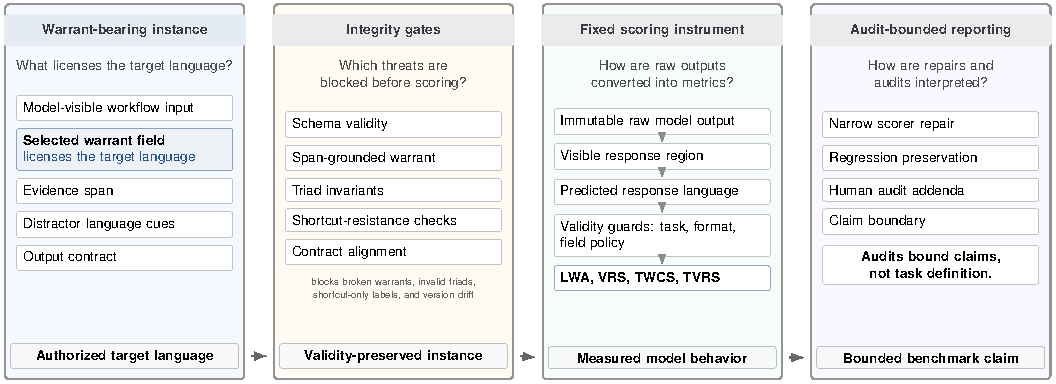
\includegraphics[width=\textwidth]{figures/fig3_traceable_evaluation_chain.pdf}
\caption{Traceable evaluation chain for language-warrant evaluation. \dataset{} treats the selected warrant field, integrity gates, scoring instrument, and audit boundary as inspectable parts of the benchmark artifact.}
\label{fig:traceable-evaluation-chain}
\end{figure*}

Figure~\ref{fig:traceable-evaluation-chain} summarizes the evaluation chain used for the frozen release. The first stage defines the warrant-bearing instance. It records the model-visible workflow input, selected warrant field, evidence span, distractor language cues, and output contract. These fields determine which language is authorized for the response. The second stage applies integrity gates before scoring. These gates check schema validity, span-grounded warrants, triad invariants, shortcut-resistance conditions, and contract alignment. They prevent broken warrants, invalid triads, shortcut-only labels, and version drift from entering the reported measurements.

The third stage fixes the scoring instrument. Raw model outputs are preserved, the visible response region is extracted, the predicted response language is identified, and validity guards are applied before metric aggregation. The fourth stage bounds reporting. Scorer repair, regression checks, and human audit addenda support the final metric freeze, but they do not redefine the task. This separation makes each wrong-language decision traceable to the prompt, selected warrant, visible output region, and scorer decision.

\subsection{Scoring contract}

The scorer operates on the user-visible natural-language region of each model output. This region is separated from structured fields, internal notes, or machine-readable payloads whose language policy may differ from the recipient-facing surface. The predicted language of the visible region is then compared with the target language licensed by the selected warrant field. In parallel, the scorer records task completion, format compliance, and field-language policy compliance. These guard scores prevent language-following metrics from crediting empty, malformed, or contract-violating outputs.


For item $i$, let $y_i$ be the authorized target language derived from the selected warrant, and let $\hat{y}_i$ be the predicted language of the scored visible region. The item-level authorized-language indicator is
\begin{equation}
a_i = \mathbf{1}\{\hat{y}_i = y_i\}.
\label{eq:item-authorized-language}
\end{equation}

Authorized language following is the mean of this indicator over the evaluated item set $\mathcal{I}$:
\begin{equation}
\mathrm{LWA} =
\frac{1}{|\mathcal{I}|}
\sum_{i\in\mathcal{I}} a_i .
\label{eq:lwa}
\end{equation}

Let $\mathrm{TC}_i$, $\mathrm{FMT}_i$, and $\mathrm{FLP}_i$ denote task completion, format compliance, and field-language policy compliance. The guarded valid-response score for item $i$ is
\begin{equation}
\mathrm{VRS}_i =
a_i
\cdot
\mathrm{TC}_i
\cdot
\mathrm{FMT}_i
\cdot
\mathrm{FLP}_i .
\label{eq:vrs-item}
\end{equation}
We report \metric{VRS} as the mean of $\mathrm{VRS}_i$ over $\mathcal{I}$. Thus, \metric{LWA} measures whether the response language is authorized, while \metric{VRS} additionally requires task completion, format compliance, and field-policy compliance.

At the triad level, let $g=(b,w,d)$ denote the base, warrant-shift, and distractor-shift items. Valid triads satisfy two structural conditions before scoring: the warrant-shift item changes the authorized target language, $y_w \neq y_b$, and the distractor-shift item preserves it, $y_d = y_b$. For a valid triad $g$, triad-level warrant consistency is
\begin{equation}
\mathrm{TWCS}_g =
a_b
\cdot
a_w
\cdot
a_d .
\label{eq:twcs-item}
\end{equation}

The aggregate triad-level warrant-consistency score is
\begin{equation}
\mathrm{TWCS} =
\frac{1}{|\mathcal{G}|}
\sum_{g\in\mathcal{G}} \mathrm{TWCS}_g ,
\label{eq:twcs}
\end{equation}
where $\mathcal{G}$ is the set of valid triads. The stricter triad-level valid-response score requires all three items in the triad to satisfy the guarded valid-response contract:
\begin{equation}
\mathrm{TVRS}_g =
\mathrm{VRS}_b
\cdot
\mathrm{VRS}_w
\cdot
\mathrm{VRS}_d .
\label{eq:tvrs-item}
\end{equation}
We report \metric{TVRS} as the mean of $\mathrm{TVRS}_g$ over $\mathcal{G}$. Together, \metric{LWA}, \metric{VRS}, \metric{TWCS}, and \metric{TVRS} separate item-level language authorization, guarded response validity, triad-level warrant consistency, and guarded triad validity. Because \metric{TWCS} is a conjunctive triad score, it is not interpreted through the raw arithmetic gap \(\mathrm{LWA}-\mathrm{TWCS}\). For calibration, we also use a descriptive item-rate baseline,
\begin{equation}
\mathrm{TWCS}_{\mathrm{ind}} = \mathrm{LWA}^{3},
\label{eq:twcs-ind}
\end{equation}
which is the expected triad pass rate under identical independent item-level correctness. This baseline is not a behavioral null model. It prevents overinterpreting the natural shrinkage caused by requiring all three items in a triad to pass.


\subsection{Scorer Repair and Metric Freeze}

The final paper metrics use the frozen v0.2k scorer as the fixed scoring instrument. This scorer was introduced after a targeted human audit identified a systematic language undercrediting failure mode, before the final main-result interpretation was frozen. The repair was deliberately narrow: it updated the language scoring component and the positive triad relation constraints supported by the audit evidence, while preserving the dataset, raw model outputs, model identities, task completion scoring, format scoring, and field policy scoring. The repair was therefore a scorer-correctness update, not a model-ranking or result-optimization step.

We verified the repair by replaying the audited records against the repaired scorer. The v0.2k scorer matched 312 of 312 audited item records and 286 of 286 audited triad records, with zero item mismatches and zero triad mismatches. A separate regression replay then checked that the official-main artifacts used the same dataset and raw outputs, and that non-language guard scores were not redefined by the repair. We therefore use v0.2k as an audited benchmark instrument for the paper's main language warrant claims. This does not make the scorer a fully automatic ground truth oracle. It means that the reported metrics are computed by a fixed instrument whose language scoring repair was checked against the human audit evidence available for the final release.

\begin{table}[t]
\centering
\caption{Audit evidence for the final scoring instrument.}
\label{tab:audit-governance-summary}
\scriptsize
\setlength{\tabcolsep}{2.6pt}
\renewcommand{\arraystretch}{1.08}
\begin{tabularx}{\columnwidth}{@{}>{\raggedright\arraybackslash}p{0.25\columnwidth}>{\raggedright\arraybackslash}p{0.20\columnwidth}>{\raggedright\arraybackslash}p{0.22\columnwidth}>{\raggedright\arraybackslash}X@{}}
\toprule
\textbf{Check} & \textbf{Unit} & \textbf{Result} & \textbf{Supported claim} \tabularnewline
\midrule
Repair replay & 312 items; 286 triads & 0 item and 0 triad mismatches & v0.2k language scorer matches audited repair evidence \tabularnewline
Regression replay & six official-main runs & dataset, raw outputs, and guard scores preserved & final metrics are computed from unchanged run artifacts \tabularnewline
External-flag audit & 72 flagged rows & VRS: 58 agreements; 14 conservative auto scores; 0 lenient auto scores & external-audit flags do not inflate guarded validity claims \tabularnewline
Second-auditor overlap & 70 rows, score-blind & language agreement = 0.957; $\kappa=0.844$ & primary language judgments have stronger support than strict format/VRS judgments \tabularnewline
Rule-focused adjudication & 63 disagreement rows, de novo & format and VRS remain rubric-sensitive & guarded validity is reported conservatively and separately from LWA/TWCS \tabularnewline
\bottomrule
\end{tabularx}
\end{table}

Table~\ref{tab:audit-governance-summary} summarizes the evidence used to fix and bound the final scoring instrument. The strongest support is for language warrant measurement: the repaired scorer exactly replays the audited item and triad records, and the regression replay preserves the dataset, raw outputs, and non-language guard scores across the six official-main runs. The additional audits limit overclaiming by checking flagged rows, score-blind overlap, and rule-focused adjudication cases. They also show why \metric{LWA} and \metric{TWCS} are the primary response-language authorization metrics, while \metric{VRS} and \metric{TVRS} remain conservative guarded metrics whose strict format and valid-response components have lower audit agreement.


\section{Experimental Setup}

\subsection{Evaluation Object and Leakage Control}

We evaluate all models on the frozen 1,500-instance release described in Section~III, which consists of 500 controlled warrant triads. For each item, the model receives only the \texttt{model\_visible\_input} field. All evaluator-only metadata is withheld, including the target response language, selected warrant field, warrant statement, evidence spans, language-following rule, task-completion rule, format rule, and field-language policy. This zero-metadata setting tests whether the model can recover the operative response-language warrant from the workflow prompt itself, rather than from benchmark-specific annotations.

This separation is central to the benchmark construct. The model-visible prompt may contain several plausible language-bearing fields, but only one field or policy element licenses the response language for the current task. Revealing the selected warrant, the gold language, or the scoring rule would convert the benchmark from warrant recovery into ordinary instruction following. We therefore use hidden metadata only for scoring and slice analysis.

\subsection{Model Runs and Generation Protocol}

All \emph{official-main} runs use the same prompt construction. The model-visible workflow input is passed directly to the model, without additional language reminders, warrant hints, chain-of-thought requests, demonstrations, or benchmark-specific instructions. Each run records one raw completion per item. The run artifact stores the input hash, run identifier, model name, model provider or local path, decoding configuration, prompt-construction tag, and timestamp. Generation is deterministic where supported, with one completion per item, temperature zero, top-p one, and a maximum output budget of 512 tokens.

The official-main comparison contains six full-1500 runs: Claude Sonnet 4.6, Aya Expanse 8B, Gemini 3.5 Flash, Llama-3.1-8B-Instruct, GPT-5.5, and Qwen3-8B-Instruct. These are the only runs used in the main model-comparison tables. Additional runs are retained only for boundary checks: Mistral-7B-Instruct-v0.3 is a full-1500 diagnostic run, GPT-5.5 xhigh is a sensitivity run, and Gemini 3.1 Pro Preview is a 300-item diagnostic slice. These runs are reported separately when relevant and are not pooled with the official-main comparison.

API and local-model runs are normalized at the artifact level rather than during generation. Raw outputs are preserved before scoring, and all item-level, triad-level, and slice-level scores are computed afterward using the same frozen v0.2k scorer. This design keeps model generation, raw-output preservation, and metric computation as separate stages, which allows the reported results to be regenerated from the released artifacts.

\subsection{Scoring and Reporting Plan}

The scoring pipeline follows Section~IV. For each raw output, the scorer extracts the user-visible response region, predicts the language of that region, applies task-completion and format guards, checks field-language policy when applicable, and aggregates item scores into triad scores. The primary item-level measures are \metric{LWA} and \metric{VRS}. The primary triad-level measures are \metric{TWCS} and \metric{TVRS}. Task completion, format compliance, and field-language policy compliance are reported as guard metrics, not as substitutes for authorized language following.

The analysis is organized around four research questions. RQ1 measures how much authorized response-language following varies across the six official-main models and reports uncertainty intervals for the two headline language metrics. RQ2 calibrates triad-level warrant consistency against item-level language following without treating the raw item-to-triad arithmetic difference as a standalone diagnostic, then decomposes the triad into base, warrant-shift, and distractor-shift behavior. RQ3 localizes the main paper failures by difficulty level, warrant-source family, structured-output condition, and shortcut-cue pressure. Fine-grained field paths and individual pattern IDs remain in the artifact release because many cells are too small for main-paper claims. RQ4 uses diagnostic and sensitivity runs only to bound interpretation. This organization keeps the experiment focused on response-language authorization under competing workflow cues, rather than presenting \dataset{} as a general-purpose model leaderboard.


\section{Results}
\suppressfloats[t]

This section reports the official-main results on the frozen 1,500-instance release. The analysis uses model comparisons to test the benchmark construct, not to establish a general-purpose leaderboard. The central question is whether a model binds the response language to the workflow evidence that authorizes it when several plausible language cues are visible.

\subsection{RQ1. Authorized response-language following}

\begin{table}[t]
\caption{Official-main headline results.}
\label{tab:official-main-results}
\centering
\scriptsize
\setlength{\tabcolsep}{2.7pt}
\renewcommand{\arraystretch}{1.08}
\begin{tabular}{@{}lrrrrr@{}}
\toprule
\textbf{Model} &
\textbf{TC} &
\textbf{LWA} &
\textbf{TWCS} &
\boldmath$\mathrm{LWA}^{3}$ &
\boldmath$\mathrm{Excess}_{\mathrm{ind}}$ \tabularnewline
\midrule
GPT-5.5 & 0.961 & \textbf{0.989} & \textbf{0.968} & 0.966 & 0.002 \tabularnewline
Gemini 3.5 Flash & 0.967 & 0.824 & 0.702 & 0.559 & 0.143 \tabularnewline
Claude Sonnet 4.6 & 0.958 & 0.690 & 0.458 & 0.329 & 0.129 \tabularnewline
Qwen3-8B-Inst. & \textbf{0.981} & 0.462 & 0.276 & 0.099 & 0.177 \tabularnewline
Aya Expanse 8B & 0.955 & 0.413 & 0.218 & 0.070 & 0.148 \tabularnewline
Llama-3.1-8B & 0.900 & 0.301 & 0.108 & 0.027 & 0.081 \tabularnewline
\bottomrule
\end{tabular}

\vspace{0.25em}
\begin{minipage}{0.96\columnwidth}
\scriptsize
TC is task completion; LWA is authorized language following; TWCS is triad warrant consistency. $\mathrm{LWA}^{3}$ is the descriptive independent-item baseline from Eq.~\ref{eq:twcs-ind}; $\mathrm{Excess}_{\mathrm{ind}}=\mathrm{TWCS}-\mathrm{LWA}^{3}$. Rows are sorted by TWCS.
\end{minipage}
\end{table}

\begin{table}[t]
\caption{Wilson 95\% intervals for headline language metrics.}
\label{tab:headline-ci}
\centering
\scriptsize
\setlength{\tabcolsep}{3.8pt}
\renewcommand{\arraystretch}{1.06}
\begin{tabular}{@{}lcc@{}}
\toprule
\textbf{Model} & \textbf{LWA 95\% CI} & \textbf{TWCS 95\% CI} \tabularnewline
\midrule
GPT-5.5 & [0.982, 0.993] & [0.949, 0.980] \tabularnewline
Gemini & [0.804, 0.842] & [0.660, 0.740] \tabularnewline
Claude & [0.666, 0.713] & [0.415, 0.502] \tabularnewline
Qwen3 & [0.437, 0.487] & [0.239, 0.317] \tabularnewline
Aya & [0.388, 0.438] & [0.184, 0.256] \tabularnewline
Llama & [0.279, 0.325] & [0.084, 0.138] \tabularnewline
\bottomrule
\end{tabular}
\vspace{0.25em}
\begin{minipage}{0.95\columnwidth}
\scriptsize
Intervals treat item-level LWA as a binomial proportion over 1,500 items and TWCS as a binomial proportion over 500 triads. Model names are abbreviated for width.
\end{minipage}
\end{table}

Table~\ref{tab:official-main-results} reports the headline official-main comparison. The table is intentionally restricted to the metrics needed for the main contrast: task completion, item-level authorized language following, triad-level warrant consistency, and a calibrated item-rate baseline for the conjunctive triad score. Full guarded-validity behavior is analyzed through the slice profile in Fig.~\ref{fig:level-slice-profile}. Table~\ref{tab:headline-ci} adds Wilson intervals for the two headline language metrics. The large gaps among the top, middle, and weaker runs exceed the uncertainty induced by finite item and triad counts, while close comparisons within a narrow band should not be overinterpreted without additional repeated-generation evidence.

The main pattern is not a conventional model-ranking effect. Task completion remains high across all official-main runs, but authorized language following and triad-level warrant consistency separate sharply. \metric{TWCS} ranges from 0.108 to 0.968, showing that completing the workflow task does not imply satisfying the controlled warrant pattern. The clearest separations are between task completion and triad consistency: Qwen3-8B-Inst. completes 0.981 of items but reaches only 0.276 \metric{TWCS}, and Llama-3.1-8B completes 0.900 of items but reaches only 0.108 \metric{TWCS}.

This separation supports the central premise of \dataset{}: response-language authorization is a workflow evidence-selection problem. A model can understand the task and produce a nonempty, task-relevant response while still grounding the response language in the wrong visible cue. The strongest run remains near ceiling at both the item and triad levels, while lower-performing runs reveal that task completion alone substantially overstates workflow-language reliability. The calibrated columns in Table~\ref{tab:official-main-results} also show why the raw difference between LWA and TWCS is not used as a primary diagnostic: much of that difference follows mechanically from the conjunctive triad definition.


\subsection{RQ2. Item-level scores and triad-level consistency}

Item-level and triad-level metrics test different aspects of reliability. \metric{LWA} asks whether an individual output uses the language authorized by its selected warrant. \metric{TWCS} asks whether the model preserves the required behavior across a controlled triad: it must follow the base warrant, change language when the warrant changes, and remain stable when only a distractor cue changes.

The triad metric is intentionally conjunctive, so it will usually be lower than item-level accuracy even when item errors are independent. For this reason, Table~\ref{tab:official-main-results} reports \(\mathrm{LWA}^{3}\) as a descriptive item-rate calibration. The comparison is useful in two ways. First, it separates the strictness of the triad score from the behavioral claim. A low \metric{TWCS} is meaningful because it is low in absolute workflow terms, not because \(\mathrm{LWA}-\mathrm{TWCS}\) is large. Second, the positive \(\mathrm{TWCS}-\mathrm{LWA}^{3}\) values show that triad outcomes are not simply random independent item successes; some models pass or fail in correlated groups, as expected under shared workflow and warrant structure.

Table~\ref{tab:role-counterfactual-diagnostics} decomposes the triad into its three item roles and two relation checks. The role columns show that the item-level difficulty is not concentrated in only one row of the triad: for each model, base, warrant-shift, and distractor-shift LWA stay in the same broad band. The relation columns are stricter. Warrant-shift success (WSS) requires the model to change language when the selected warrant changes, while distractor-invariance success (DIS) requires the model to preserve the authorized language when only a non-authoritative cue changes. These two checks expose the counterfactual structure that item-level LWA cannot express.

\begin{table}[t]
\caption{Role-level and counterfactual relation diagnostics.}
\label{tab:role-counterfactual-diagnostics}
\centering
\scriptsize
\setlength{\tabcolsep}{3.3pt}
\renewcommand{\arraystretch}{1.06}
\begin{tabular}{@{}lrrrrr@{}}
\toprule
\textbf{Model} & \textbf{Base} & \textbf{Warr.} & \textbf{Dist.} & \textbf{WSS} & \textbf{DIS} \tabularnewline
\midrule
GPT-5.5 & 0.984 & 0.988 & 0.994 & 0.972 & 0.980 \tabularnewline
Gemini & 0.824 & 0.824 & 0.824 & 0.744 & 0.768 \tabularnewline
Claude & 0.696 & 0.684 & 0.690 & 0.542 & 0.572 \tabularnewline
Qwen3 & 0.452 & 0.472 & 0.462 & 0.310 & 0.388 \tabularnewline
Aya & 0.408 & 0.412 & 0.418 & 0.254 & 0.324 \tabularnewline
Llama & 0.306 & 0.284 & 0.314 & 0.118 & 0.248 \tabularnewline
\bottomrule
\end{tabular}
\vspace{0.25em}
\begin{minipage}{0.96\columnwidth}
\scriptsize
Base, Warr., and Dist. are item-level LWA for the base, warrant-change, and distractor-change roles. WSS is warrant-shift success; DIS is distractor-invariance success. Each role has 500 items per model; each relation has 500 triads per model.
\end{minipage}
\end{table}

The main RQ2 finding is therefore conservative. \metric{TWCS} should not be read as a transformed version of \metric{LWA}. It asks whether item-level authorized-language behavior survives the two counterfactual requirements of the triad. GPT-5.5 is near the calibrated item-rate ceiling, while several weaker runs remain low in absolute triad reliability despite high task completion. Thus, the value of the triad metric is construct control: it tests sensitivity to warrant-relevant edits and invariance to warrant-irrelevant edits within the same workflow group.

\subsection{RQ3. Failure concentration across benchmark slices}

\begin{figure*}[t]
\centering
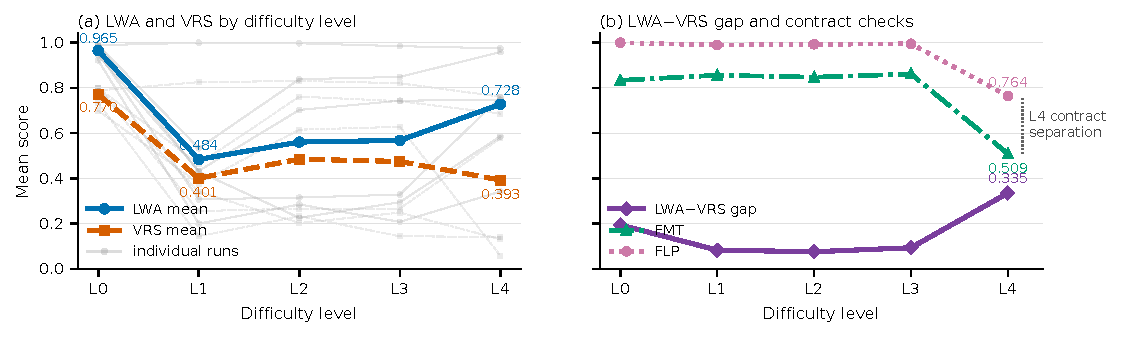
\includegraphics[width=\textwidth]{figures/fig4_level_slice_profile.pdf}
\caption{Difficulty-level slice profile across the six official-main runs. Panel (a) compares authorized language following (LWA) and valid response score (VRS) from L0 to L4, with gray traces showing individual runs. Panel (b) shows the LWA and VRS separation together with format compliance (FMT) and field-language policy compliance (FLP), highlighting the L4 contract-separation effect.}
\label{fig:level-slice-profile}
\end{figure*}


\begin{table}[t]
\centering
\caption{Official-main high-level slice contrasts.}
\label{tab:slice-contrasts}
\scriptsize
\setlength{\tabcolsep}{3.0pt}
\renewcommand{\arraystretch}{1.06}
\begin{tabularx}{\columnwidth}{@{}>{\raggedright\arraybackslash}p{0.42\columnwidth}rrrrr@{}}
\toprule
\textbf{Slice} & \textbf{Items} & \textbf{LWA} & \textbf{VRS} & \textbf{FMT} & \textbf{FLP} \tabularnewline
\midrule
L0 direct instruction & 90 & 0.965 & 0.770 & 0.833 & 1.000 \tabularnewline
L1--L3 workflow-mediated & 1,050 & 0.544 & 0.460 & 0.855 & 0.993 \tabularnewline
L4 structured contract & 360 & 0.728 & 0.393 & 0.509 & 0.764 \tabularnewline
No structured output & 1,122 & 0.577 & 0.492 & 0.867 & 1.000 \tabularnewline
Structured output & 378 & 0.720 & 0.374 & 0.485 & 0.755 \tabularnewline
\bottomrule
\end{tabularx}
\vspace{0.25em}
\begin{minipage}{0.98\columnwidth}
\scriptsize
Values are item-weighted means over the six official-main runs. Structured output is defined by a non-null structured-output type in the release metadata.
\end{minipage}
\end{table}

Fig.~\ref{fig:level-slice-profile} and Table~\ref{tab:slice-contrasts} show that failures are not distributed uniformly across difficulty levels or output-contract types. Direct language instructions at L0 are substantially easier than workflow-mediated warrants. Once the operative language must be inferred from recipient, policy, profile, channel, or route evidence, performance drops and remains in a harder regime across L1 to L3.

Table~\ref{tab:warrant-source-slices} further separates the workflow-mediated cases by warrant-source family. Explicit language instructions are easiest. The hardest main family is customer response locale, where the authorized language is present as workflow metadata rather than as a direct final-response instruction. Policy-selected contact locale and active outbound surface sit in the middle. Schema-visible locale policy has higher LWA but much lower VRS because it combines language selection with structured field and format obligations.

\begin{table}[t]
\centering
\caption{Warrant-source slice performance.}
\label{tab:warrant-source-slices}
\scriptsize
\setlength{\tabcolsep}{2.6pt}
\renewcommand{\arraystretch}{1.06}
\begin{tabularx}{\columnwidth}{@{}>{\raggedright\arraybackslash}p{0.47\columnwidth}rrrr@{}}
\toprule
\textbf{Warrant source} & \textbf{Items} & \textbf{LWA} & \textbf{VRS} & \textbf{TC} \tabularnewline
\midrule
Explicit instruction & 90 & 0.965 & 0.770 & 0.954 \tabularnewline
Customer response locale & 243 & 0.469 & 0.401 & 0.975 \tabularnewline
Policy-selected contact locale & 351 & 0.566 & 0.499 & 0.965 \tabularnewline
Active outbound surface & 351 & 0.550 & 0.476 & 0.933 \tabularnewline
Schema-visible locale policy & 324 & 0.722 & 0.360 & 0.947 \tabularnewline
Other field-level locale & 141 & 0.661 & 0.482 & 0.956 \tabularnewline
\bottomrule
\end{tabularx}
\vspace{0.25em}
\begin{minipage}{0.98\columnwidth}
\scriptsize
Items count the frozen dataset rows in each family. Metric values are item-weighted means over the six official-main runs.
\end{minipage}
\end{table}

The benchmark also checks whether simple visible-cue heuristics could solve the task. Table~\ref{tab:shortcut-baselines} reports metadata-only shortcuts computed from the frozen gold labels. Following the operator language, source/material language, audience language, or majority target language is far below all official-main model LWA values except in trivial comparison to the weakest model's lower range. This supports the construct claim: successful performance requires identifying the authorized warrant, not merely copying a salient language-bearing field.

\begin{table}[t]
\centering
\caption{Static shortcut-cue baselines from dataset metadata.}
\label{tab:shortcut-baselines}
\scriptsize
\setlength{\tabcolsep}{4.0pt}
\renewcommand{\arraystretch}{1.06}
\begin{tabularx}{\columnwidth}{@{}>{\raggedright\arraybackslash}p{0.70\columnwidth}rr@{}}
\toprule
\textbf{Shortcut rule} & \textbf{Items} & \textbf{Gold match} \tabularnewline
\midrule
Follow operator language & 1,500 & 0.015 \tabularnewline
Follow source/material language & 1,500 & 0.044 \tabularnewline
Follow audience language & 1,500 & 0.173 \tabularnewline
Always majority target language (English) & 1,500 & 0.129 \tabularnewline
\bottomrule
\end{tabularx}
\vspace{0.25em}
\begin{minipage}{0.98\columnwidth}
\scriptsize
Gold match is the fraction of dataset items for which the shortcut-selected language equals the authorized target language.
\end{minipage}
\end{table}

L4 has a different profile. Authorized language following improves relative to the middle levels, but guarded validity drops. The drop is concentrated in the guard components rather than in task completion: the L4 mean \metric{FMT} is 0.509 and \metric{FLP} is 0.764, while \metric{TC} remains 0.952. Panel (b) explains this pattern: structured-output items introduce additional contract checks beyond selecting the correct recipient-facing language. Failures therefore shift from pure warrant selection toward schema conformance, visible/internal field separation, and field-level language policy compliance.

This slice profile supports three interpretations. First, direct language instructions are not an adequate proxy for workflow-mediated language warrants. Second, warrant-source families matter: customer and policy metadata, active surfaces, and schema-visible locale policies produce different failure profiles. Third, structured-output settings add a separate guarded-validity burden. \metric{LWA} and \metric{VRS} should therefore remain distinct: one measures authorized language selection, while the other also reflects whether the output satisfies the surrounding workflow contract.

\subsection{RQ4. Diagnostic and sensitivity runs}

Diagnostic and sensitivity runs are not part of the official-main comparison. They are used only to bound interpretation. The artifact release includes two scored non-main full-1500 runs under the same frozen v0.2k scoring instrument: a Mistral-7B-Instruct-v0.3 diagnostic run and a GPT-5.5 xhigh reasoning sensitivity run. Table~\ref{tab:diagnostic-sensitivity-runs} reports these runs together with the official GPT-5.5 row as a reference point.


\begin{table}[t]
\centering
\caption{Boundary checks outside the official main comparison.}
\label{tab:diagnostic-sensitivity-runs}
\footnotesize
\setlength{\tabcolsep}{4.5pt}
\renewcommand{\arraystretch}{1.08}
\begin{tabularx}{\columnwidth}{@{}>{\raggedright\arraybackslash}p{0.42\columnwidth}>{\raggedright\arraybackslash}p{0.20\columnwidth}ccc@{}}
\toprule
\textbf{Run} & \textbf{Role} & \textbf{TC} & \textbf{LWA} & \textbf{TWCS} \tabularnewline
\midrule
GPT-5.5 & Official reference & 0.961 & 0.989 & 0.968 \tabularnewline
GPT-5.5 xhigh & Sensitivity & 0.959 & 0.975 & 0.938 \tabularnewline
Mistral-7B-v0.3 & Diagnostic & 0.959 & 0.356 & 0.150 \tabularnewline
\bottomrule
\end{tabularx}
\vspace{0.25em}
\begin{minipage}{0.98\columnwidth}
\footnotesize
All rows contain 1,500 items and use the frozen v0.2k scoring instrument. Only GPT-5.5 is part of the official main comparison.
\end{minipage}
\end{table}



The Mistral diagnostic run follows the weaker-model pattern observed in the official-main comparison: task completion remains high, but response-language authorization and triad-level warrant consistency remain low. Its \metric{TC} is 0.959, while \metric{LWA} is 0.356 and \metric{TWCS} is 0.150. This reinforces the main finding that task completion and language-warrant selection are separable behaviors.

The GPT-5.5 xhigh reasoning run provides a sensitivity check for the strongest official model. It remains close to the official GPT-5.5 run, but it does not improve the primary language-warrant metrics. Relative to official GPT-5.5, \metric{LWA} decreases from 0.989 to 0.975, and \metric{TWCS} decreases from 0.968 to 0.938. The result suggests that increasing reasoning effort does not by itself eliminate the need to identify the authoritative workflow evidence for response language.

These diagnostics do not change the primary empirical basis of the paper. The six official-main runs remain the basis for model-level claims. The additional scored full-1500 runs instead provide boundary evidence: the weak-run pattern recurs for an adjacent open model, and the strongest-model pattern is stable under a nearby reasoning configuration. A separate 300-item Gemini Pro Preview raw-output diagnostic is retained in the release artifacts, but it is not scored under the final metric tables and is not used for paper claims.


\subsection{Summary of findings}

The results support four conclusions. First, high task completion does not solve response-language authorization: models can complete the workflow task while failing to bind the response language to the authorized evidence. Second, controlled triads add information beyond item-level language correctness by testing whether models respond to warrant-relevant changes while resisting warrant-irrelevant cue changes. Third, simple shortcut rules are insufficient: operator-language, source-language, audience-language, and majority-language shortcuts match the authorized target language only 0.015, 0.044, 0.173, and 0.129 of items, respectively. Fourth, failures are slice-dependent: direct language instructions are easy, workflow-mediated warrant-source families are substantially harder, and structured-output settings introduce additional format and field-policy failures beyond language following.


\section{Discussion and Limitations}

\subsection{What \dataset{} measures}
\dataset{} evaluates response-language authorization under controlled workflow cue conflict. Its target is therefore distinct from general multilingual capability or ordinary instruction-following accuracy. A model may recognize all languages in the prompt, complete the task, and still fail the benchmark by binding the response language to a non-authoritative evidence item. This distinction is central to the empirical results. The strongest runs show that the task is feasible, while the weaker runs show that workflow evidence selection remains fragile even when task completion is high.

The triad design makes this distinction observable. Item-level authorized language following indicates that the model produced the expected response language for one instance. Triad-level warrant consistency imposes a stronger behavioral requirement: the model should follow the original warrant, change language when the warrant changes, and remain stable when only a shortcut cue changes. Because this score is conjunctive, its raw difference from item-level accuracy is not itself a causal estimate of shortcut following. Its value is that it evaluates the controlled group pattern that single-item language accuracy cannot test.

\subsection{Implications for multilingual workflow evaluation}
The central lesson of \dataset{} is that response-language reliability in multilingual workflows depends on evidence selection, not only on generation quality. Practical prompts often expose several language-bearing fields at once, including user turns, source records, internal notes, customer profiles, channel policies, locale metadata, and output schemas. Treating these visible cues as equivalent obscures the authority structure of the task. \dataset{} makes this structure explicit by asking which evidence item licenses the response language.

This view changes how multilingual robustness should be evaluated. First, task completion should be separated from warrant-consistent output. A response can be useful, well formed, and semantically relevant while still using an unauthorized language. Second, robustness should be tested with counterfactual controls rather than with isolated items alone. A model that appears correct on one item may be following a shortcut cue. Warrant-shift and distractor-shift controls are needed to distinguish sensitivity to the selected warrant from robustness against salient but non-authoritative cues.

\subsection{Implications for workflow system design}
The benchmark also identifies system-design pressure points. Workflow systems often encode response-language authority in metadata fields, policy records, locale fields, routing decisions, or schema-visible contracts. When this authority is implicit in a long prompt, a model may bind the response language to a more salient cue. Explicit warrant extraction, clearer separation between user-visible and internal fields, schema-level locale policies, and post-generation language validation are natural intervention points. These are design implications suggested by the benchmark, rather than evidence that any particular prompting strategy or system architecture resolves the problem.

The results further caution against treating stronger general models as uniformly reliable workflow agents. The best official-main run performs well, but the model spread is large, and several runs maintain high task completion while failing warrant consistency. Deployment evaluations should therefore include workflow-specific controls when response language has user-facing, contractual, compliance, or policy-sensitive consequences.

\subsection{Validity boundaries}
The main construct is language-warrant selection. \dataset{} operationalizes this construct through selected warrant fields, evidence spans, shortcut cues, warrant-shift controls, distractor-shift controls, and triad-level scores. This operationalization captures observable warrant-consistent behavior under controlled perturbations. It is a behavioral measure, not direct evidence of the model's internal causal reasoning. A model may produce a warrant-consistent triad pattern through an explicit authority representation, through a learned heuristic, or through some other policy that happens to match the controlled triad. Conversely, an isolated wrong output may reflect decoding variation, formatting behavior, mixed-script output, quoted text, or language-identification ambiguity rather than a stable shortcut-following strategy.

The release controls several internal-validity risks through frozen instance identifiers, preserved raw outputs, fixed scorer contracts, regression-verified v0.2k scoring, targeted audit materials, and follow-up scorer addenda. These controls reduce the risk that the reported findings arise from dataset drift, post hoc metric changes, or untracked scorer behavior. Some measurement risks remain. Visible-output extraction and language identification are harder for short spans, structured payloads, mixed scripts, quoted material, and responses containing both internal and user-facing text. For this reason, the paper treats \metric{LWA} and \metric{TWCS} as the primary authorization measures, while \metric{VRS} and \metric{TVRS} serve as conservative guarded measures that additionally require valid task responses. The released records are constructed workflow-style instances, not live customer records, and the benchmark does not include real account credentials, private addresses, or production access tokens. Authorization in this paper means authorization under the benchmark workflow contract, not legal authority over real users or institutions.

\subsection{Scope of generalization}
\dataset{} is a controlled benchmark rather than a sample of natural enterprise traffic. It covers eight target languages, five difficulty levels, multiple warrant-source families, workflow-style task settings, and structured-output variants. This coverage is sufficient for evaluating the proposed construct, but real deployments may involve additional languages, dialects, organizations, policy regimes, schema families, communication channels, and interaction histories. The benchmark should therefore be interpreted as a controlled test of response-language authorization, rather than as a complete certificate of multilingual workflow reliability.

The official-main comparison uses six full-1500 runs under a shared protocol. This is sufficient to show that current models differ sharply on the benchmark construct, but it is not a comprehensive leaderboard over all available models, decoding strategies, system prompts, tool-using agents, or repeated-sampling policies. The protocol evaluates one completion per item to make the main comparison reproducible and auditable. Future evaluations can add repeated runs, prompt-paraphrase robustness, agentic tool settings, and intervention tracks that expose or require the selected warrant explicitly.

\subsection{Benchmark release and future extensions}
The frozen release is intended as an evaluation instrument for language-warrant selection. Its main value lies in the controlled triad structure, auditable warrant provenance, and scorer contracts that make response-language authorization measurable. Future versions can expand in several directions: broader language and dialect coverage, more diverse schema families, privacy-preserving abstractions of naturalistic workflow logs, repeated-sampling protocols, and intervention tracks for explicit warrant extraction, schema compilers, policy-aware prompting, and post-generation validation.

These extensions should preserve the central control principle. Additional realism is useful when warrant-relevant changes remain distinguishable from shortcut-cue changes. The contribution of \dataset{} is therefore not limited to its current templates or language set. It provides an evaluation design for measuring whether a model binds response language to the workflow evidence that authorizes it.


\section{Conclusion}

This paper introduced \dataset{}, a benchmark for evaluating response-language authorization in multilingual workflow prompts. The benchmark targets a failure mode that ordinary target-language accuracy does not isolate: a model can complete the visible task, generate a plausible response, and still bind the response language to a salient but non-authoritative cue. \dataset{} makes this failure measurable through 1,500 instances organized as 500 controlled warrant triads, where warrant shifts should change the authorized language and distractor shifts should not.

The official-main evaluation shows that response-language authorization is a distinct and uneven capability among the evaluated LLMs. Across six full-1500 runs, task completion remains at or above 0.900, while triad-level warrant consistency ranges from 0.108 to 0.968. This divergence shows why multilingual workflow evaluation should separate task completion, item-level authorized language following, and triad-level warrant consistency. Language-bearing context should therefore not be treated as a flat set of cues; only some visible fields license the response language for the current workflow action.

Beyond the empirical results, \dataset{} contributes an auditable evaluation instrument for this setting. Selected warrant fields, licensing evidence spans, shortcut roles, triad roles, and fixed scorer contracts make response-language authority inspectable rather than implicit. The broader implication is that multilingual workflow evaluation should audit which evidence authorizes an output language, not merely whether the output appears in a plausible language.


\section*{Artifact Availability}

The anonymous review artifact contains the frozen 1,500-instance release, 500 blueprint groups, run manifests, raw-output inventories, item-level and triad-level metric tables, scorer-governance notes, human-audit addenda, checksum manifests, analysis scripts, and paper figures. The paper-facing benchmark name is \dataset{}; frozen item identifiers and some filenames retain the legacy \texttt{SLD\_v1\_0} prefix to preserve release hashes and provenance. The public release will add the repository URL, license, and archival DOI selected by the authors.

\section*{AI-Generated Content Acknowledgement}

The authors used OpenAI ChatGPT based on GPT-5.5 Thinking as a writing and editing assistant during paper preparation, including prose revision, LaTeX issue checking, table and figure iteration, and artifact-report drafting. The authors reviewed and edited the generated material and are responsible for the final benchmark data, experimental results, analysis, and claims.


\bibliographystyle{IEEEtran}
\bibliography{references}

\end{document}
